%!TEX root =../cmbs4_scibook.tex 
%%%%%% CMB-S4 BSM Physics Chapter  %%%%%%%%%%%%%%%%

% This was created by Renee Hlozek from text in the inflation and neutrino sections

\chapter{Physics Beyond The Standard Model}

In addition to constraints on primordial parameters in the standard 6-parameter model, and a detection of (or upper limits on) the scalar-to-tensor ratio, CMB-S4 will yield unprecedented constraints on interesting physics beyond the standard picture. 

\section{Constraints on Axion-like particles}
The QCD axion and other axion-like particles (ALPs), if stable on cosmological timescales, can contribute to the DM density. Along with thermal WIMPs, they are a well-motivated DM candidate (see Ref.~\cite{Marsh:2015xka} for a recent review).

Non-thermally produced ultralight axions (ULAs) with masses in the range $10^{-33}~{\rm eV}\leq m_{a}\leq 10^{-20}~{\rm eV}$ are well motivated by string theory, can contribute to either the dark matter or dark energy components of the Universe, depending on their masses, and are distinguishable from DE and CDM in cosmological observables. The current best constraints from the primary CMB TT power, and WiggleZ galaxy redshift survey were made in \cite{hlozek:2015axa}. Our fiducial axion energy density is chosen to be consistent with these constraints. 
\subsection{Constraints on the axion energy density}
The degeneracies of the axions with other cosmological parameters, such as $N_\mathrm{eff}$ or $m_\nu$, vary depending on the axion mass (see Fig.~\ref{fig:axions}, right panel). Dark energy-like axions with masses around $10^{-33}~{\rm eV}$ change the late-time expansion rate and therefore the sound horizon, changing the location of the acoustic peaks. This has degeneracies with the matter and curvature content. 
Heavier axions ($m_a \gtrsim 10^{-26}~{\rm eV}$) affect the expansion rate in the radiation era and reduce the angular scale of the diffusion distance, leading to a boost in the higher acoustic peaks, which has a degeneracy with $N_{\rm eff}$. 

In both of these cases, improved errors on the temperature and polarization power spectrum, coupled with constraints on the Hubble constant (for the lightest axions) from Baryon Acoustic Oscillations, lead to improvements in the error on allowed axion energy density of a factor of three from these spectra alone. 

In the matter power spectrum, and thus CMB lensing power, light axions suppress clustering power, suggesting a degeneracy with effects of massive neutrinos that must be broken to make an unambiguous measurement of neutrino mass using the CMB. The above-mentioned effects in the expansion rate break this degeneracy for some axion masses. There remains a significant degeneracy between axions and massive neutrinos $m_a=3\times 10^{-29}\text{ eV}$ and $\Sigma m_\nu=60\text{ meV}$. Effort should be made to break this degeneracy and distinguish the effects of non-thermal axions from massive neutrinos for an unambiguous detection of neutrino mass using the CMB. 

\begin{figure}[t] 
\begin{center} 
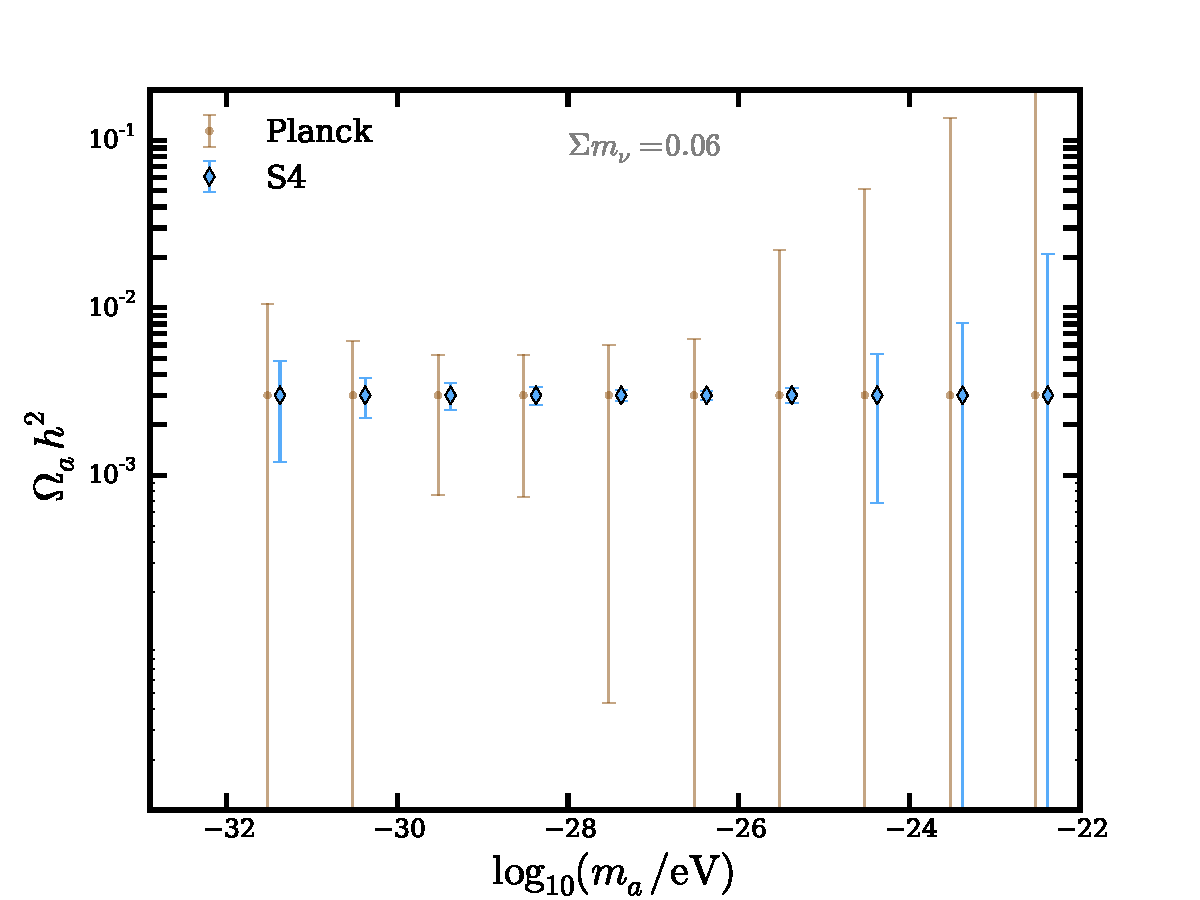
\includegraphics[width=0.49\textwidth]{DarkEnergy/Log_constraints_axions_s4.pdf}
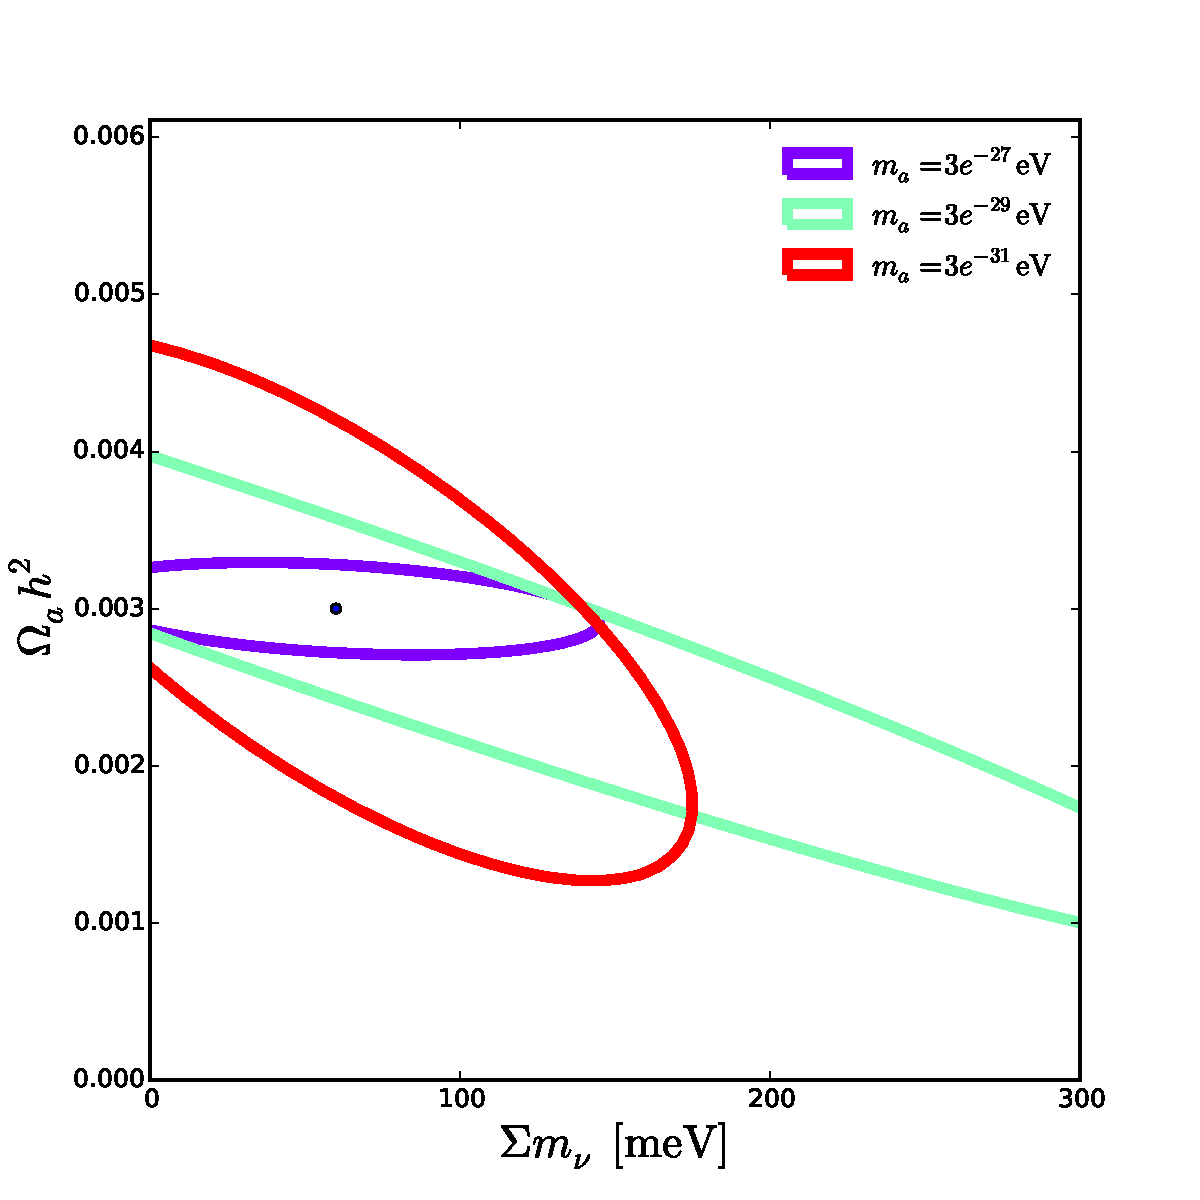
\includegraphics[width=0.49\textwidth]{DarkEnergy/s4_omnuh2_omaxh2_allmass.pdf}
\caption{(\textit{Left:} Constraints on the axion energy density as a function of axion mass at fixed neutrino mass $\Sigma m_\nu = 0.06~\rm{eV}$. Over the `fuzzy' dark matter region, S4 allow for percent-level constraints on an axion component, improving significantly on current constraints. \textit{Right:} Degeneracy of axions with massive neutrinos. There is a significant degeneracy for $m_a=3\times 10^{-29}\text{ eV}$ and $\Sigma m_\nu=60\text{ meV}$.
\label{fig:axions}}
\end{center}       
\end{figure}       

We show the forecasted constraints on the axion energy density from S4 including lensing in the left panel of Figure~\ref{fig:axions} (for fixed neutrino mass of $\Sigma m_\nu = 0.06~\rm{eV}$). Adding in information from the lensing reconstruction using S4 will improve constraints on axion DM significantly. A percent-level measurement of the lensing deflection power at multipoles $\ell > 1000$ leads to an improvement in the error on the axion energy density of a factor of eight relative to the current Planck constraints, for an axion mass of $m_a=10^{-26}~{\rm eV}$.    This represents an ability to test the component nature of dark matter, and thus the CDM paradigm, at the percent level. Furthermore, since $\Omega_a\propto f_a^2$ this improves the expected constraint on the axion decay constant from $10^{17}\text{ GeV}$ with Planck to $10^{16}\text{ GeV}$ with S4, testing the predictions of the ``string axiverse’’ scenario~\cite{axiverse}. 

For higher mass axions there is a strong degeneracy between CDM and axions. Using high-$\ell$ lesing measurements, S4 breaks this degeneracy at larger masses than Planck. However, this degeneracy is still significant and care should be taken in interpreting the constraints on the energy density shown in Fig.~\ref{fig:axions}. Constraints at $m_a\gtrsim 10^{-24}\text{ eV}$ are driven by the improved measurement of the total matter density, and do not allow one to distinguish such axions from CDM at high precision.  Achieving further improvement in the mass constraint will require improved understanding of non-linear clustering of axions. These constraints represent the absolute lower bound on DM particle mass from cosmology. If this bound can be improved and the degeneracy broken up to $10^{-23}\text{ eV}$, the CMB will begin to make contact to the ``Fuzzy DM’’ axion model~\cite{hu:00a, marsh:2013js}. 


\subsection{Axion Isocurvature}

A key axion parameter is the symmetry breaking scale, $f_a$. If $H_I/2\pi<f_a$, the axion DM acquires \emph{uncorrelated isocurvature perturbations} (e.g. Refs.~\cite{Axenides:1983hj,Fox:2004kb,Hertzberg:2008wr}).\footnote{We ignore the case where $H_I/2\pi>f_a$, since no isocurvature initial conditions are excited. The limit $r_{0.05}<0.12$ implies that isocurvature is produced if $f_a>1.8\times 10^{13}\text{ GeV}$. This accounts for the QCD axion in the ``anthropic'' window (roughly half of the allowed range of $f_a$ on a logarithmic scale), axions with GUT scale decay constants (such as string axions~\cite{Svrcek:2006yi,Arvanitaki:2009fg}) and axions with lower $f_a$ in models of low-scale inflation.} The uncorrelated CDM isocurvature amplitude is bounded by \emph{Planck} to be $A_I/A_s<0.038$ at 95\% C.L.~\cite{Ade:2015lrj}. We performed a forecast for CMB-S4: the isocurvature limit will be improved by a factor of approximately five compared to \emph{Planck}, allowing for detection of axion-type isocurvature at 2$\sigma$ significance in the region $0.008<A_I/A_s<0.038$.

The axion isocurvature amplitude is:
\begin{equation}
A_I = \left(\frac{\Omega_a}{\Omega_d}\right)^2\frac{(H_I/M_{\rm pl})^2}{\pi^2(\phi_i/M_{\rm pl})^2} \, .
\label{eqn:iso_amplitude}
\end{equation}
The initial axion displacement, $\phi_i$, fixes the axion relic abundance such that $\Omega_a=\Omega_a (\phi_i,m_a)$~\cite{Preskill:1982cy,Abbott:1982af,Dine:1982ah,Turner:1983he,Steinhardt:1983ia,Marsh:2010wq}. Thus, if the relic density and mass can be measured by independent means, \emph{a measurement of the axion isocurvature amplitude can be used to measure the energy scale of inflation, $H_I$}

If the QCD axion is all of the DM, axion direct detection experiments can be used in conjunction with CMB-S4 to probe $H_I$ in the range
\begin{equation}
 2.5\times 10^6\lesssim H_I/\text{GeV}\lesssim 4\times 10^9\, 
\text{(QCD axion + direct detection)}\, \,
\end{equation}
This is demonstrated in Fig.~\ref{fig:qcd_isocurvature} (left panel) for the case of ADMX~\cite{Asztalos:2009yp} (in operation), and CASPEr~\cite{Budker:2013hf} (proposed), where we have used the standard formulae relating the QCD axion mass and relic abundance to the decay constant (e.g. Ref.~\cite{Fox:2004kb}).\footnote{In simple models of inflation, the high-$f_a$ QCD axion is incompatible with detection of tensor modes~\cite{Fox:2004kb,Hertzberg:2008wr,Visinelli:2014twa,Marsh:2014qoa,Visinelli:2014twa}, although non-standard cosmic thermal histories of PQ breaking mechanisms can lift constraints , e.g. \cite{Higaki:2014ooa,Fairbairn:2014zta,Nomura:2015xil}.} \emph{Combining axion DM direct detection with CMB-S4 isocurvature measurements allows a unique probe of low-scale inflation, inaccessible to searches for tensor modes.}

\begin{figure*}[htbp!]
\begin{center}
$\begin{array}{@{\hspace{-0.8in}}c@{\hspace{+0.2in}}c@{\hspace{-0.5in}}}
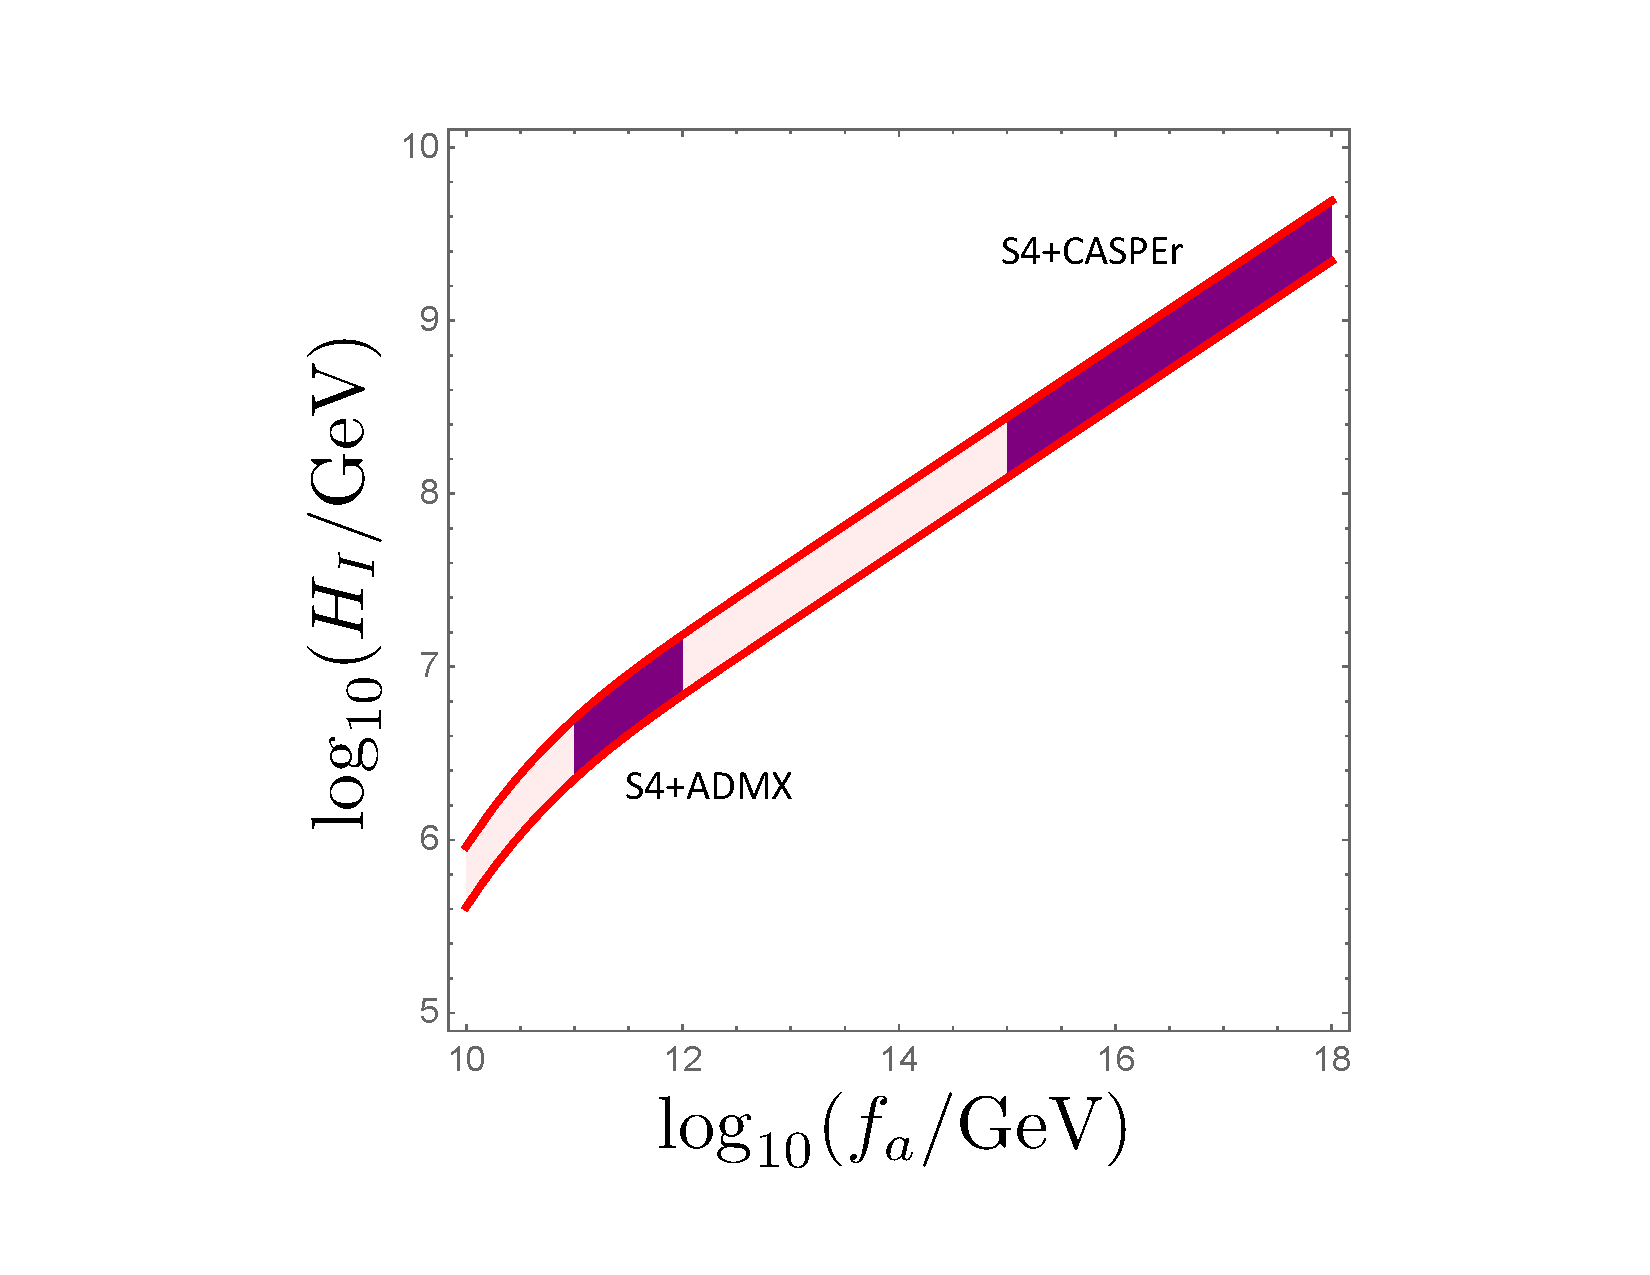
\includegraphics[width=0.4\textwidth]{Inflation/admx_casper_labelled.pdf} &
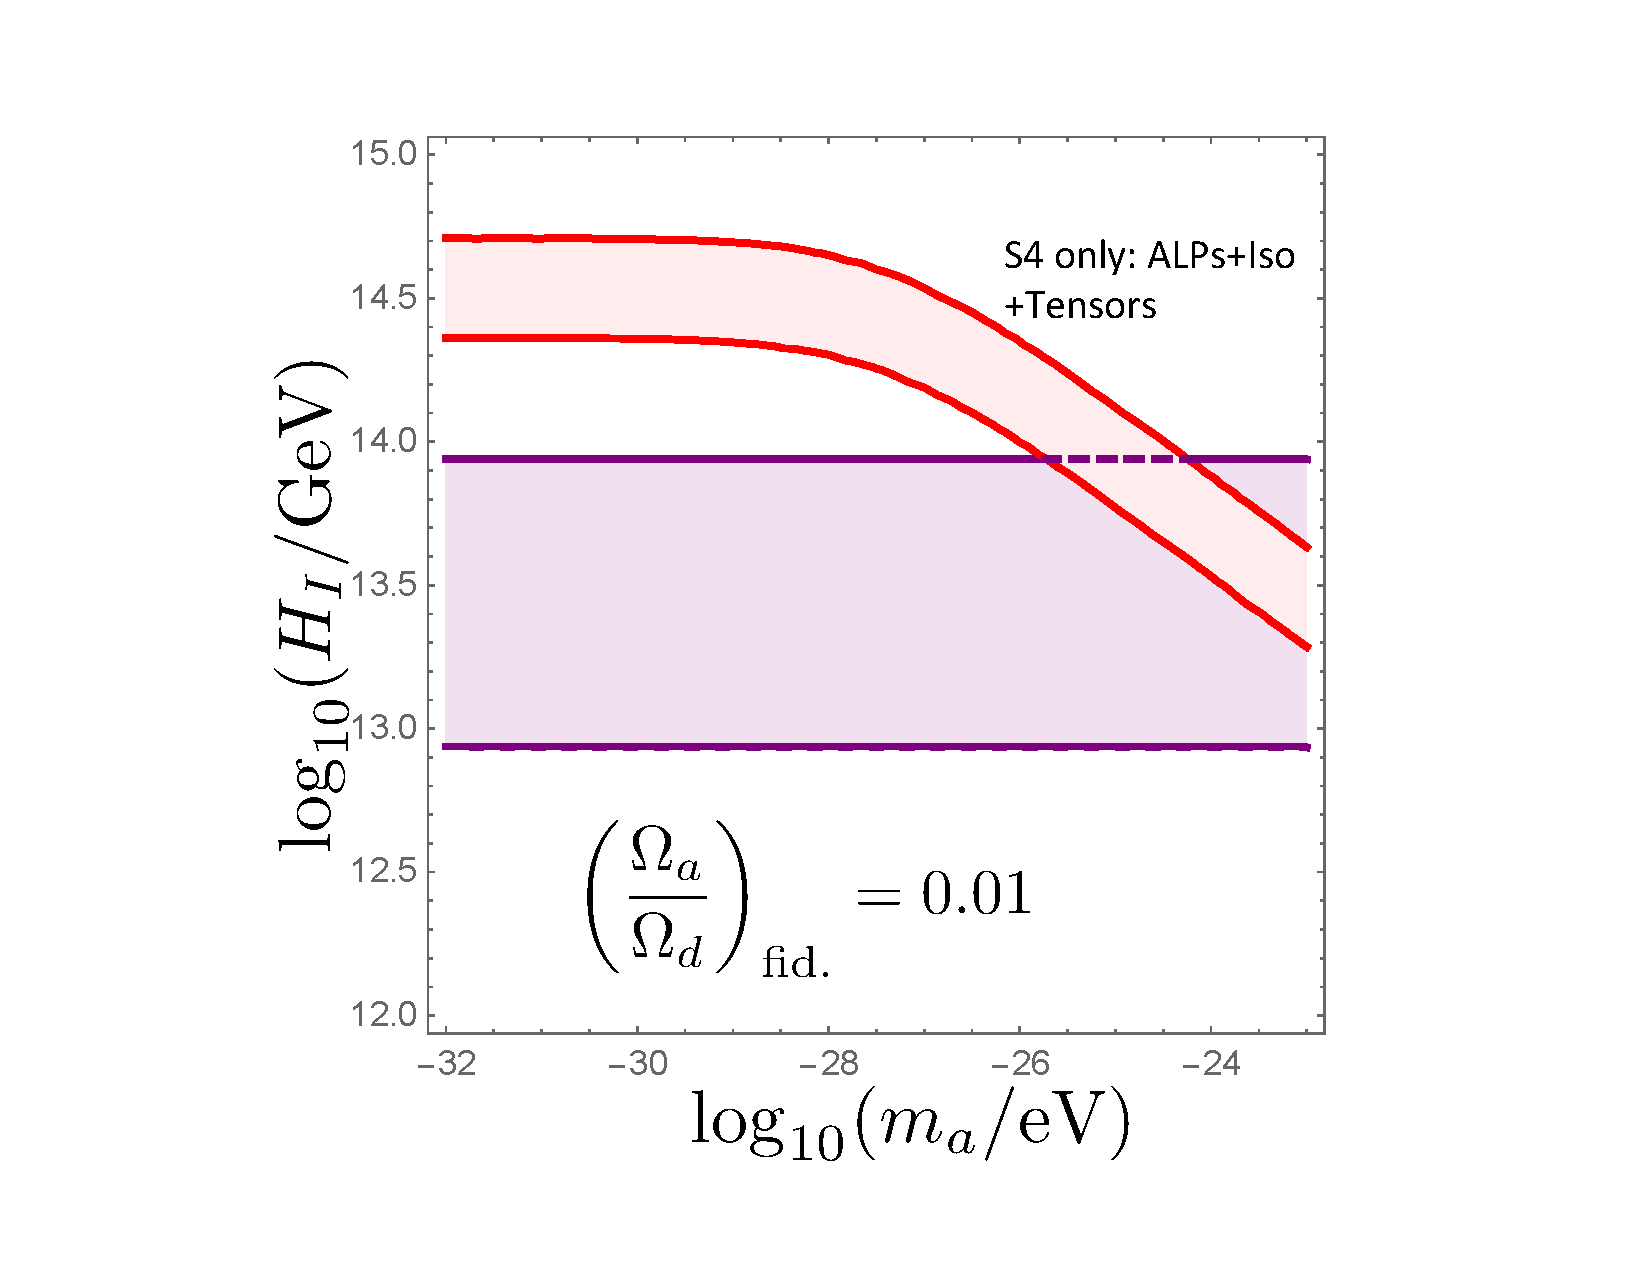
\includegraphics[width=0.4\textwidth]{Inflation/alp_iso_labelled.pdf}
 \end{array}$
 \end{center}
 \caption{Axion dark matter isocurvature. Red bands shows isocurvature amplitude consistent with \emph{Planck} and detectable with S4. \emph{Left Panel} The QCD axion: measuring the energy scale of inflation with S4+axion direct detection. Here we restrict axions to be all of the DM. The purple regions show the range of $f_a$ accessible to axion direct detection experiments. Combining ADMX~\cite{Asztalos:2009yp} (in operation), CASPEr~\cite{Budker:2013hf} (proposed), and S4 it is possible to measure $4\times 10^5\lesssim H_I/\text{GeV}\lesssim 4\times 10^9$. \emph{Right Panel} ALPs: a combination measurement using S4 alone. Assuming 1\% of the total DM resides in an ultralight axion, the mass and axion density can be determined to high significance using, for example, the lensing power. The isocurvature amplitude can also be determined, allowing for an independent determination of $H_I$ in the same regime as is accessible from tensor modes (purple band).}
\label{fig:qcd_isocurvature}
\end{figure*} 
We now consider isocurvature in ultralight ALPs (ULAs, see e.g. Refs.~\cite{Marsh:2013taa,Marsh:2014qoa}). ULA DM has a number of distinctive features in large scale structure and the CMB~\cite{Hlozek:2015axa,Marsh:2013ywa}. For ULAs with $10^{-32}\lesssim m_a/\text{eV}\lesssim 10^{-23}$ a DM fraction of $\Omega_a/\Omega_d$ in the range of 1\% is consistent with \emph{Planck}~\cite{Hlozek:2015axa} and high-$z$ galaxy formation~\cite{Bozek:2014uqa,Schive:2015kza}, yet can be distinguished from pure CDM using S4 lensing power at $>2\sigma$ (depending on the ULA mass, Sec.~\ref{sec:uladiabat}). Fig.~\ref{fig:qcd_isocurvature} (right panel) shows isocurvature constraints possible with S4, compared to tensor constraints. We fix the fiducial ULA fraction to 1\%, such that $\Omega_a$ and $m_a$ can be separately measured using the S4 lensing power, and thus using Eq.~(\ref{eqn:iso_amplitude}) a measurement of $A_I$ is a measurement of $H_I$. 

In contrast to the QCD axion, there are masses, $m_a\lesssim 10^{-26}\text{ eV}$, for which tensor modes impose a stronger constraint on $H_I$ than isocurvature (such that isocurvature in these ALPs would be undetectably small). However, there are also regions of overlap between possible tensor and isocurvature measurements. Using S4 in these regions, it is possible to make a combination measurement of isocurvature and axion parameters, giving an independent measurement of $H_I$:
\begin{equation} 2.5\times 10^{13}\lesssim H_I/\text{GeV}\lesssim 10^{14}\,
\text{(ultralight ALPs, S4 alone)}\,\,.
\end{equation}
This applies to ALPs in the mass range $10^{-26}\lesssim m_a/\text{eV}\lesssim 10^{-23}$, where effects on lensing of a 1\% axion fraction can be distinguished from CDM. \emph{Detecting isocurvature and lensing effects from ULAs using CMB-S4 can provide a measurement of $H_I$ complementary to searches for tensor modes.}%\footnote{We note that obtaining a 1\% fraction in such ALPs requires $f_a\gg 1.8\times 10^{13}\text{ GeV}$, and so isocurvature in ULA DM is guaranteed.}


\subsection{Constraints on Axion couplings}

%A ubiquitous component of extensions of the Standard Model are axions and/or axion-%like particles (ALPs).  Axions have been introduced to solve the strong-CP problem~%\cite{Peccei:1977hh}, the hierarchy problem~\cite{Graham:2015cka}, and the %naturalness problem of inflation~\cite{Freese:1990rb}.  Furthermore, they appear %generically in string theory in large numbers, leading to the qualitative phenomena %described as the string axiverse~\cite{Arvanitaki:2009fg}.

%ALPs typically appear as (pseudo)-Goldstone bosons of some high energy global %symmetry.  At low energy, the mass of the ALP is protected by an approximate shift %symmetry of the general form $a \to a + c$ where $a$ is the axion and $c$ is a %constant (for non-abelian Goldstone bosons, this transformation will include higher %order terms in $a$).  We will define an ALP to be any (pseudo)-scalar particle for %which all couplings to the Standard Model respect such a symmetry.  This symmetry %may be softly broken with an explicit mass term, although this is highly restricted %in the case of the QCD axion.

Two couplings of particular interest for axion phenomenology are the coupling to gluons and photons, 
\beq
\frac{1}{4} g_{a \gamma \gamma} a \tilde F_{\mu \nu}F^{\mu\nu} \ , \qquad \qquad \frac{1}{4} g_{a g g} a \tilde G_{\mu \nu}G^{\mu\nu}  \ .
\eeq
These couplings typically appear as the consequence of chiral anomalies.  The coupling of the axion to gluons is what makes the solution to the strong-CP problem possible.  The coupling to photons is somewhat model dependent but typically arises in conjunction with the gluon coupling.  In addition to or instead of these couplings, a variety of other possible couplings to matter may also be included.

\begin{figure}[h!]
\centering 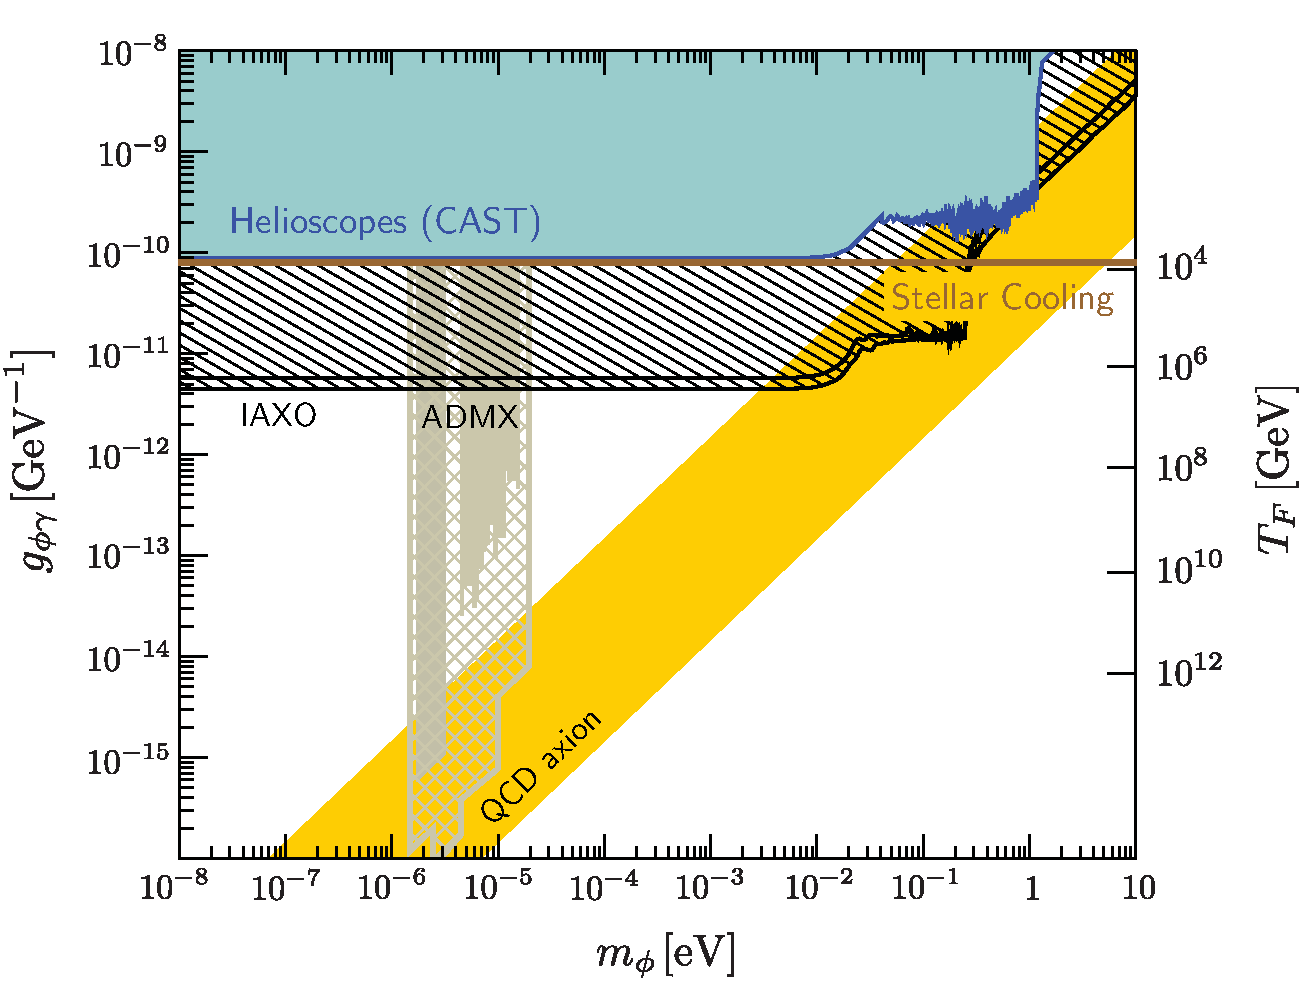
\includegraphics[width=0.70\textwidth]{Neutrinos/AxionPhotonWithFuture.pdf}
\caption{Relationship between freeze-out temperature ($T_F$) and axion-photon coupling ($g_{a\gamma\gamma}$).  While freeze-out is independent of the mass, experimental probes of the coupling are strongly mass dependent.  For $T_F > 10^4$~GeV the axion coupling would predict $\Delta \Neff = 0.027$.  Sensitivity to $\Delta\Neff$ at that level would translate into sensitivity to axions with $T_F \leq T_{\rm reheat}$.  For plausible values of $T_{\rm reheat} > 10^{10}$~GeV, cosmology is orders of magnitude more sensitive than existing bounds over a wide range of masses.}
\label{fig:axionphoton}
\end{figure}

Two very common features of models containing ALPs are that the ALPs are typically light (in many cases, $m \ll 1$~eV) and their interactions are suppressed by powers of the (typically large) decay constant $f_a$.  These two features make ALPs a particularly compelling target for cosmology (and $\Neff$ specifically).  Because of the small masses, they will often behave as relativistic species in the early universe.  Furthermore, because their production rate will scale as $T^{2n +1} / f_a^{2n}$ for some $n \geq 1$, they are likely to be thermalized at high temperatures.  Given that $\Delta \Neff > 0.027$ under such circumstances, a CMB experiment with sensitivity at this level will be sensitive to a very wide range of ALP models.

The coupling of axions to matter has an additional feature that it can bring axions into thermal equilibrium at low temperatures.  Specifically, the lowest dimension coupling of an axion to charged matter takes the form
\beq
{\cal L} = -\frac{\partial_\mu a}{\Lambda_\psi}  \bar \psi_i ( \gamma^\mu g^{ij}_V + g_A^{ij} \gamma^5 ) \psi_j
\eeq
where $\psi_{i}$ is any of the charged fermions of the Standard Model and $i,j$ label the three generations of fermions of with the same charges.  Above the scale of electroweak symmetry breaking (EWSB), this coupling leads to an abundance of axions with $\Delta \Neff = 0.027$.  Through freeze-out, we are again very sensitive to $g_V$ and $g_A$ at levels that vastly exceed current limits.  In addition, below the scale of EWSB, this coupling can bring the axions into thermal equilibrium at low temperatures (freeze-in) below the mass of the heaviest fermion, $T_F \lesssim m_{3}$.  Freeze-in will produce $\Delta \Neff \approx 0.05$ and is therefore easier to detect.  For reheating temperatures well above the electroweak scale, the sensitivity of freeze-out exceeds that of freeze-in, although both are far more sensitive than current limits on axion couplings to  second and third generation fermions.

The coupling to matter is motivated also by the approximate $U(3)^5$ flavor symmetry of the Standard Model.  It is natural for such couplings to arise if the axion is a goldstone boson that results from spontaneous breaking of this symmetry (or a sub-group).  Given the non-abelian nature of the flavor symmetry, these scenarios can often lead to many axions (also known as familons).  Under such circumstances, the contribution to freeze-out is given by 
\beq
\Delta \Neff = N_a \times 0.027
\eeq
where $N_a$ is the number of axions / number of broken generators of the symmetry group.  It is easy to find scenarios where $N_a\sim {\cal O}(10)$ which is at the current level of sensitivity.


{\it Status of current observations} -- Current constraints on ALPs arise from a combination of experimental~\cite{Graham:2015ouw}, astrophysical~\cite{Raffelt:2012kt}, and cosmological~\cite{Marsh:2015xka} probes.  Current cosmological constraints are driven by several effects that depend on the mass of the axion.  For axion masses greater than 100 eV, stable thermal ALPs are easily excluded because they produce dark matter abundances inconsistent with observations.  By including the free-streaming effects of thermal QCD-axions,  Planck data~\cite{DiValentino:2015wba} combined with local measurements provide the constrain $m_a < 0.525$ eV (95 \% CL).  At larger masses, ALPs become unstable and can be constrained by the change to $\Neff$ from energy injection as well as from spectral distortions and changes to BBN~\cite{Cadamuro:2011fd,Follin:2015hya}.

{\it Implications for CMB Stange IV} -- Sensitivity to $\Delta \Neff =0.027$ is sufficient to probe the entire mass range of ALPs down to $m_a =0$ under the assumption that it thermalized in the early universe.  Interpreting such bounds in terms of the couplings of axions is more complicated~\cite{Brust:2013xpv} and can depend on assumptions about the reheating temperature.  For high (but plausible) reheat temperatures of $10^{10}$ GeV, CMB stage IV would be sensitive to $g_{a\gamma \gamma}, \, g_{a g g} \,  < \, 10^{-13} {\rm GeV}^{-1}$~\cite{Baumann:2016wac} as illustrated in figures~\ref{fig:axionphoton} and~\ref{fig:axiondipole}.  These projected limits exceed current constraints and future probes for a range of possible axion masses (including the QCD axion).

The implications for the couplings to matter are similar for the contribution from freeze-out.  However, the freeze-in contribution of $\Delta \Neff \gtrsim 0.05$ would be easier to exclude experimentally, but still produces the limits~\cite{Baumann:2016wac}
\beq
\Lambda_{\psi_i}  \ >\ \left\{ \begin{array}{ll} \displaystyle 1.3\times 10^8 \, {\rm GeV} \left(\frac{g_{*,i}}{g_{*,\tau}}\right)^{\!-1/4} \left(\frac{m_i}{m_\tau}\right)^{\!1/2} & \quad i=\text{leptons}, \\[10pt]
\displaystyle 2.1\times 10^9 \, {\rm GeV} \left(\frac{g_{*,i}}{g_{*,t}}\right)^{\!-1/4} \left(\frac{m_i}{m_t}\right)^{\!1/2} & \quad i=\text{quarks}.
\end{array} \right.
\eeq
where $g_{*,i}$ is the number of degrees of freedom at temperature $T = m_i$.  For second and third generation fermions, these limits would exceed current bounds by several orders of magnitude.


\begin{figure}[h!]
\centering 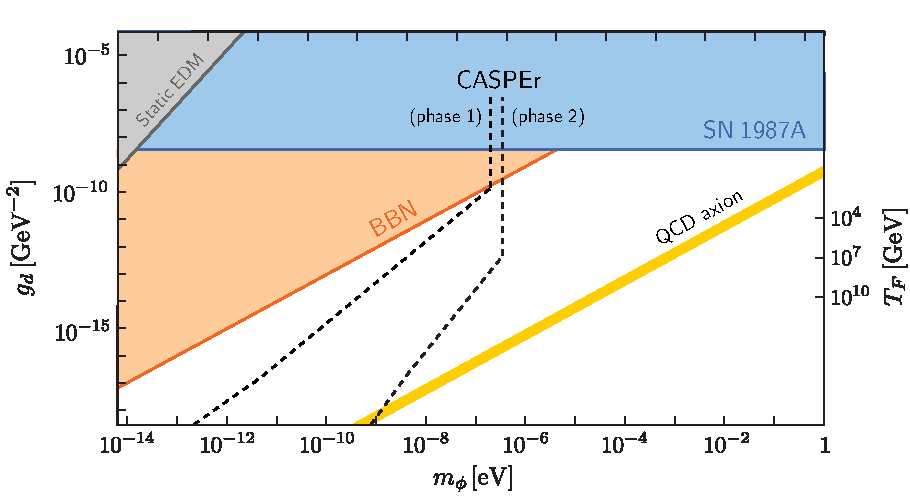
\includegraphics[width=0.70\textwidth]{Neutrinos/DipoleWithCASPErAndBBN.pdf}
\caption{Relationship between freeze-out temperature ($T_F$) and axion-gluon coupling via the neutron dipole ($g_d$).  While freeze-out is independent of the mass, experimental probes of the coupling are strongly mass dependent. We see that cosmology is more sensitive than current limits even for freeze-out temperatures below the eletro-weak phase transition and therefore could be probed by $\Delta \Neff > 0.027$.   }
\label{fig:axiondipole}
\end{figure}

\section{Spatial Curvature}

Despite the fact that inflation drives the spatial curvature to zero at the level of the background evolution, it predicts small, but non-zero curvature for a typical observer. The curvature measured in a Hubble patch receives contributions from long wavelength perturbations and is expected to be $|\Omega_k|<10^{-4}$. A measurements of $\Omega_k$ exceeding this expectation would contain important information about the process responsible for inflation. In particular, if $|\Omega_k|$ is found to be considerably larger than this value, it would tell us that the inflaton was not slowly rolling when scales slightly larger than our observable horizon exited the horizon. Furthermore, observations of large negative $\Omega_k$ would falsify eternal inflation, while observation of positive and large $\Omega_k$ would be consistent with false vacuum eternal inflation~\cite{Guth:2012ww,Kleban:2012ph}.

Current constraints on this parameter from the CMB alone are $\Omega_k= 0.005^{+0.016}_{-0.017}$. Including baryon acoustic oscillation (BAO) data tightens the bound to $\Omega_k=0.000\pm0.005$. CMB-S4 is expected to constrain spatial curvature at a level of $\sigma(\Omega_k)\approx 10^{-3}$. A detection at this level would have profound implications for the inflationary paradigm. 



\section{Microwave Background Anomalies}

Several unexpected features have been observed in the temperature of the CMB sky at relatively low-l or large angular scales.  Some of these were first noticed in COBE data,  
and all have been seen in both WMAP and Planck maps.  These include: 
\begin{itemize}
  \item a lack of correlation on the largest angular scales;
  \item alignment of the lowest multipole moments with one another and with the geometry and motion of the Solar System;
 \item greater power in odd-parity modes than in even-parity ones;
  \item a hemispherical asymmetry or dipolar modulation of the power.
\end{itemize}

Compared to the expectations of the best-fit inflationary $\Lambda$CDM model, the individual p-values of these features are in the per mille to per cent level, and therefore each anomaly has a frequentist probability at approximately the 3-sigma level or higher.  Since certain pairs of anomalies are uncorrelated in $\Lambda$CDM, in combination they nominally represents a very significant detection of anomalous behaviour. 

There are however two possible concerns before one can conclude that the CMB large-angle pattern is truly anomalous. First, these features were identified a posteriori and are characterized by statistics that were devised after the anomalies were first noted. Second, there is no physical understanding of how the collection of such features could arise. In order to help address or resolve these concerns, it is therefore crucial to obtain additional information about the large-scale primordial fluctuations, and to devise a successful model or other explanation.

The observed features can have two possible origins: either our cosmological model is incomplete and requires a modification (the “new physics hypothesis”), or we just happen to live in a realization of that model that is statistically unlikely (the “fluke hypothesis”).   Meanwhile, cosmologists have effectively exhausted their ability to obtain further independent CMB temperature data that can test these anomalies, as observations are already cosmic-variance limited at the relevant angular scales.

It has been suggested that one may nevertheless make observational progress even in the absence of an alternative model.  This can occur in two ways:
\begin{enumerate}
  \item In the fluke hypothesis the conditional probability distributions of $\Lambda$CDM for correlation functions of CMB polarization
  (and other observables) with CMB temperature and with one another are altered by the observed temperature anomalies  
  (Dvorkin et al 2008, Copi et al 2013, Yoho et al. 2013). 
  \item In the new physics hypothesis, a given phenomenological model that explains the anomalies will have observational consequences
  for other observable quantities [Yoho et al. 2015]. For example, the absence of large-angle correlations in T may reflect a lack of
  long-distance correlation in a fundamental physical quantity like the potential; similarly, 
  a hemispherical asymmetry in TT power could cause a similar asymmetry in EE.
\end{enumerate}

A variety of ideas have been proposed to explain the anomalies, ranging from Solar system dust artifacts to anisotropic models of inflation (for a summary, see Copi et al, 2016). Unfortunately, none of those ideas lead to a convincing explanation, as it is simply difficult to find models that explain the alignments of the largest primordial structures in the universe while at the same time lowering the amplitude of large-angle temperature correlations (e.g. Gordon et al, 2005). 

Additional information from polarization would be of great help. To address the first three anomalies we list above would probably require a space mission, due to the need to access very low $\ell$. But CMB-S4 can shed light on the fourth one. 

CMB-S4, alone or in combination with other data, can begin to explore both the cosmological and the fluke explanation for the hemispherical power asymmetry.  For example, $\Lambda$CDM instructs us how to remove the part of the E-mode signal that is correlated to temperature; the remainder should be Gaussian random and statistically isotropic.  If it contains a hemispherical anomaly (especially one aligned with the temperature asymmetry), that would be evidence against the fluke hypothesis [Copi, Knox, O’Dwyer and Starkman, contribution to March 9/10 S4 meeting, in preparation]. 

\section{Cosmic Birefringence}
\textbf{More text to come from Vera}
The simplest dynamical way to model the accelerated expansion of the universe is to invoke a new slowly evolving scalar field that dominates its energy budget (the quintessence models for DE). Such a field generically couples to photons through the Chern-Simons term in the electromagnetic Lagrangian, causing linear polarization of photons propagating cosmological distances to rotate---the effect known as cosmic birefringence~\cite{1998PhRvL..81.3067C}. In the case of the CMB, such rotation converts the primordial E mode into B mode, producing characteristic TB and EB cross-correlations in the CMB maps \cite{2009PhRvL.102k1302K,2009PhRvD..80b3510G}. Even though there is no firm theoretical prediction for the size of this effect, if observed, it would be a clear “smoking-gun” evidence for physics beyond the standard model. Previous studies have used quadratic estimator formalism to constrain this effect \cite{2012PhRvD..86j3529G}, with the best current limit coming from sub-degree scale polarization measurements with POLARBEAR \cite{Ade:2015cao} ($<0.33$ deg$^2$ for the amplitude of a scale-invariant rotation-angle power spectrum). A promising way to pursue search for cosmic birefringence in the future is measurement of the off-diagonal EB cross correlations on small angular scales. {\bf Put in more specific predictions for S4?}

\section{Primordial Magnetic Fields}

The origin of the microgauss ($\mu$G) strength magnetic fields in galaxies and galaxy clusters is one of the long standing puzzles in astrophysics \cite{Durrer:2013pga}. It is challenging to explain such fields based solely on the dynamo mechanism, without there being some initial seed field. However, if magnetic fields were present in the early universe, they would remain frozen in the cosmic plasma and collapse with the rest of the matter to form the galactic fields \cite{Grasso:2000wj}, or at least provide the seeds for the dynamo. A primordial magnetic field (PMF) could be produced in the aftermath of cosmic phase transitions \cite{Vachaspati:1991nm} or in specially designed inflationary scenarios \cite{Turner:1987bw,Ratra:1991bn}. Detecting their signatures in the CMB temperature and polarization would decisively prove their primordial origin. Aside from explaining the galactic fields, bounds on PMF have profound implications for our understanding of the early universe.  They help constrain theories of inflation \cite{Bonvin:2011dt}, models of the QCD and electroweak phase transitions \cite{Caprini:2007xq} and baryogenesis \cite{Vachaspati:2001nb}.

A stochastic PMF affects CMB in several ways. Magnetic stress-energy induces scalar, vector and tensor mode perturbations in the metric, and the Lorentz force generates vorticity in the photon-baryon fluid \cite{Subramanian:1998fn,Mack:2001gc,Lewis:2004ef,Shaw:2009nf,Paoletti:2010rx}. Dissipation of PMF on small scales dumps energy into the plasma, which produces spectral distortions and affects the recombination history \cite{Kunze:2014eka}.  Finally, Faraday Rotation (FR) of CMB polarization converts some of the $E$-modes into $B$-modes \cite{Kosowsky:2004zh,Pogosian:2011qv}.

Stochastic PMF has two potentially observable frequency independent contributions to the $B$-mode spectrum \cite{Shaw:2009nf}. One comes from the passive, or uncompensated tensor mode, which is generated by the PMF before neutrino decoupling. For nearly scale-invariant PMF, the spectrum of this component is indistinguishable from the inflationary gravity wave signal. The amplitude of this tensor contribution is proportional to $B^4_{1\rm{Mpc}} [\ln(a_\nu / a_{\rm{PMF}})]^2$, where $B_{1\rm{Mpc}}$ is the PMF strength smoothed over $1$Mpc, $a_\nu$ is the scale factor at neutrino decoupling and $a_{\rm{PMF}}$ is the scale factor at which PMF was generated. The other is the PMF vector mode which peaks at $l \sim 2000$, with the precise peak position dependant on the PMF spectrum. The vector-mode contribution is independent of $a_{\rm{PMF}}$. 

Planck data limits the magnetic field strength to $B_{1 {\rm Mpc}}<4.4$ nanogauss (nG) at the $95\%$ confidence level \cite{Ade:2015cva}. Similar bounds were recently obtained by POLARBEAR \cite{Ade:2015cao} based on their B-mode spectrum alone.

\section{Cosmic Strings}

Cosmic strings can at most contribute O(1\%) to the total CMB temperature anisotropy~\cite{Ade:2013xla,Lizarraga:2014xza,Lazanu:2014eya}, however, they can still generate observable B-modes. As shown in \cite{Moss:2014cra}, the bounds on cosmic strings obtained solely from the POLARBEAR \cite{Ade:2014afa} and BICEP2  \cite{Ade:2014xna} B-mode spectra are comparable to those from temperature spectra. 
We forecast the predicted constraints on cosmic strings using the StringFast code \cite{Foreman:2011uj}, based on the CMBACT simulations \cite{Pogosian:1999np} of a general string network, which allows for the correlation length of the strings, the `wiggliness' (which controls the small-scale structure of the string network) and the string rms velocity. StringFast allows for fast computation of the relevant string spectra, and includes the contribution to the string spectrum from scalar, vector and tensor modes, which are most relevant for the string B-modes \cite{Foreman:2011uj}.

In keeping with the methodology of recent results, we compute the string spectrum with a value of the string tension ($G_\mu/c^2=1.97e-6$) that allows strings to make up all the TT power at $\ell=10$, and then use the fraction of the spectrum at that multipol $f_{10}$ as the forecast parameter. $f_10$ scales with the string tension as $f_{10} \propto G_\mu^2.$ The Fisher projections for Planck around a fiducial model of $f_{10}=0.01$ are $f_{10}<0.032,$ which maps to $\G_\mu/c^2 < 3.5e-7\, 95\% \mathrm{CL}$, is consistent with the Planck constraints on the AH-mimic spectra.
We assume a fidcual model for the `wiggliness' $\alpha_\mathrm{str}$, string velocity $v_\mathrm{str}$ and correlation length $\xi_\mathrm{str}$ of $1.05, 0.4$ and $0.35$ respectively, in keeping with the model assumed in \cite{Foreman:2011uj}.




CMB-S4 polawill be able to reveal the presence of cosmic strings through their B-mode signature even if strings contribute as little as 0.1\% to the CMB temperature anisotropy \cite{Avgoustidis:2011ax}. 
\textbf{Renee Hlozek to add both text and plots/tables of constraints}


